\documentclass[varwidth=true, border=2pt]{standalone}

\usepackage{pgfplots}
\usepackage{tikz}

\usetikzlibrary{calc,patterns,angles,quotes}

\begin{document}
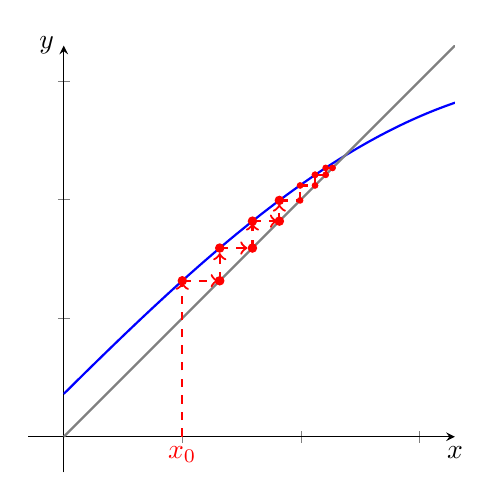
\begin{tikzpicture}
    \begin{axis}[
        legend pos=south east,
        axis x line=middle,
        axis y line=middle,
	every axis x label/.style={at={(current axis.right of origin)},anchor=north},
	every axis y label/.style={at={(current axis.above origin)},anchor=east},
	xticklabels=\empty,
	yticklabels=\empty
        grid = none ,
        width=7cm,
        height=7cm,
        grid style={dashed, gray!1},
        xmin=0,     % start the diagram at this x-coordinate
        xmax= 3,    % end   the diagram at this x-coordinate
        ymin=0,     % start the diagram at this y-coordinate
        ymax= 3,   % end   the diagram at this y-coordinate
        xlabel=$x$,
        ylabel=$y$,
        enlargelimits=true,
        tension=0.08]

        \addplot[domain=-0:8,blue, thick,samples=250] {3*cos(deg(x/3-1.45))}; % Parabola
         \addplot[domain=-0:8, gray, thick,samples=250] {x};




%	\addplot[dashed,red,mark=none] coordinates{(1,0)(1,1.316)} node[below, pos=0] {$x_0$}; %x0
%	\addplot[dashed,red,mark=none] coordinates{(1,1.316)(1.316,1.316)} node[below, pos=0] {};
%	\addplot[dashed,red,mark=none] coordinates{(1.316,1.316)(1.316,1.592)} node[below, pos=0] {};
% 	\addplot[dashed,red,mark=none] coordinates{(1.316,1.592)(1.592,1.592)} node[below, pos=0] {};
%	\addplot[dashed,red,mark=none] coordinates{(1.592,1.592)(1.592,1.819)} node[below, pos=0] {};
%	\addplot[dashed,red,mark=none] coordinates{(1.592,1.819)(1.819,1.819)} node[below, pos=0] {};
%	\addplot[dashed,red,mark=none] coordinates{(1.819,1.819)(1.819,1.994)} node[below, pos=0] {};

	\draw[red, dashed, thick, ->](axis cs: 1,0)--(axis cs:1,1.3);
	\draw[red, dashed, thick, ->](axis cs: 1,1.316)--(axis cs: 1.3,1.316);	
	\draw[red, dashed, thick, ->](axis cs: 1.316,1.316)--(axis cs: 1.316,1.55);
	\draw[red, dashed, thick, ->](axis cs: 1.316,1.592)--(axis cs: 1.55,1.592);
	\draw[red, dashed, thick, ->](axis cs: 1.592,1.592)--(axis cs: 1.592,1.8);
	\draw[red, dashed, thick, ->](axis cs: 1.592,1.819)--(axis cs: 1.8,1.819);
	\draw[red, dashed, thick, ->](axis cs: 1.819,1.819)--(axis cs: 1.819,1.96);


	\addplot[dashed,red,thick,mark=none] coordinates{(1.819,1.994)(1.994,1.994)} node[below, pos=0] {};
	\addplot[dashed,red,thick,mark=none] coordinates{(1.994,1.994)(1.994,2.12)} node[below, pos=0] {};
	\addplot[dashed,red,thick,mark=none] coordinates{(1.994,2.12)(2.12,2.12)} node[below, pos=0] {};
	\addplot[dashed,red,thick,mark=none] coordinates{(2.12,2.12)(2.12,2.21)} node[below, pos=0] {};
	\addplot[dashed,red,thick,mark=none] coordinates{(2.12,2.21)(2.21,2.21)} node[below, pos=0] {};
	\addplot[dashed,red,thick,mark=none] coordinates{(2.21,2.21)(2.21,2.268)} node[below, pos=0] {};
	\addplot[dashed,red,thick,mark=none] coordinates{(2.21,2.268)(2.268,2.268)} node[below, pos=0] {};
	
	\addplot[red, only marks, mark=*, mark size=1.5pt] coordinates {(1,1.316)(1.316,1.316)(1.316,1.592)(1.592,1.592)(1.592,1.819)(1.819,1.819)(1.819,1.994)};
	\addplot[red, only marks, mark=*, mark size=1pt] coordinates {(1.994,1.994)(1.994,2.12)(2.12,2.12)(2.12,2.21)(2.12,2.21)(2.21,2.21)(2.21,2.268)(2.268,2.268)};
	
	\node[red] (xL) at (axis cs: 1,-0.15){$x_0$};
    \end{axis}
\end{tikzpicture}
\end{document}